
\chapter{Practical Experiments}
\label{ch:inpractice}

This chapter shows two experiments and results of advanced use of the Zone. The first realises an asynchronous sequence diagram of a parallel programm with dependencies. The second describe how to transparently instrument the third-party framework \vertx\ to realize a ``Zone-aware\vertx''.

\section{Asynchronous Sequence Diagram}


\paragraph{Specifying} what is interesting in an asynchronous sequence diagram is the most complex part if this experiments. In fact, producing the information of a conventional sequence diagram is not interesting. There is already many tools to do that. The useful data is an asynchronous dependency diagram: what are the dependencies between asynchronous tasks. The produced diagram is defined by:

\begin{itemize}
\item Each task execution is divided into sub parts, represented by the nodes of a graph.
\item Task are divided into the biggest possible parts such that a sub part execution first uniquely shows \emph{incoming} dependencies (rely on other tasks result or completion). Then it uniquely shows \emph{outgoing} dependencies (another task shows incoming dependency from this task).
\item Dependencies are represented as directed edges between the corresponding nodes of their tasks.
\end{itemize}

The produced graph is a directed acyclic graph where each node represents an autonomous part of the programs and the edges shows the precedences between those parts.

\paragraph{The realization} is then pretty easy using the Zone. As evoqued in chapter \ref{ch:apps}, use the one Zone per task pattern of chapter \ref{ch:apps}, creating \lstinline{TaskZone}s. Each \lstinline{TaskZone} stores a unique task ID and define the crossing hook: 

\begin{lstlisting}
// The cross operation executes inside -destination- Zone

// The cross operation is defined inside -source- Zone

public Token crossOut(Token token) {
  TaskZone sourceZone = this;
  int sourceID = sourceZone.taskId;

  int destID = Zone.lookup(TASK_ID_KEY);

  storeDependency(souceID, destID);
}
\end{lstlisting}

The difficult part is then to compile collected information and build a graphic representation. For the code of a fork-join algorithm (figure \ref{fig:fj-alg}) I used a sample code from the d3.js library to produce the view shown in figure \ref{fig:fjt-bundle}. Each node is named 'X\#Y'. 'X' is the task id and 'Y' the subtask id. The initial task is '0', splitted in two subtasks '0\#1' entry point of algorithm and '0\#2', end of the algorithm, with output value.

\begin{figure}[h]
  \textbf{Solving problem $P$}
  \begin{enumerate}
  \item If $P$ is small then solve $P$.
  \item Else split $P$ in a list $P$s of smaller problems $p$.
  \item For each $p$ in $P$s, start an asynchronous task to solve $p$.
  \item Join each asynchronous task started in (3) and collect all sub-results.
  \item Compose the sub-results and return the final solution.
  \end{enumerate}
\caption{Generic fork-join algorithm}
\label{fig:fj-alg}
\end{figure}

\begin{figure}
  \centering
  \makebox[\textwidth][c]{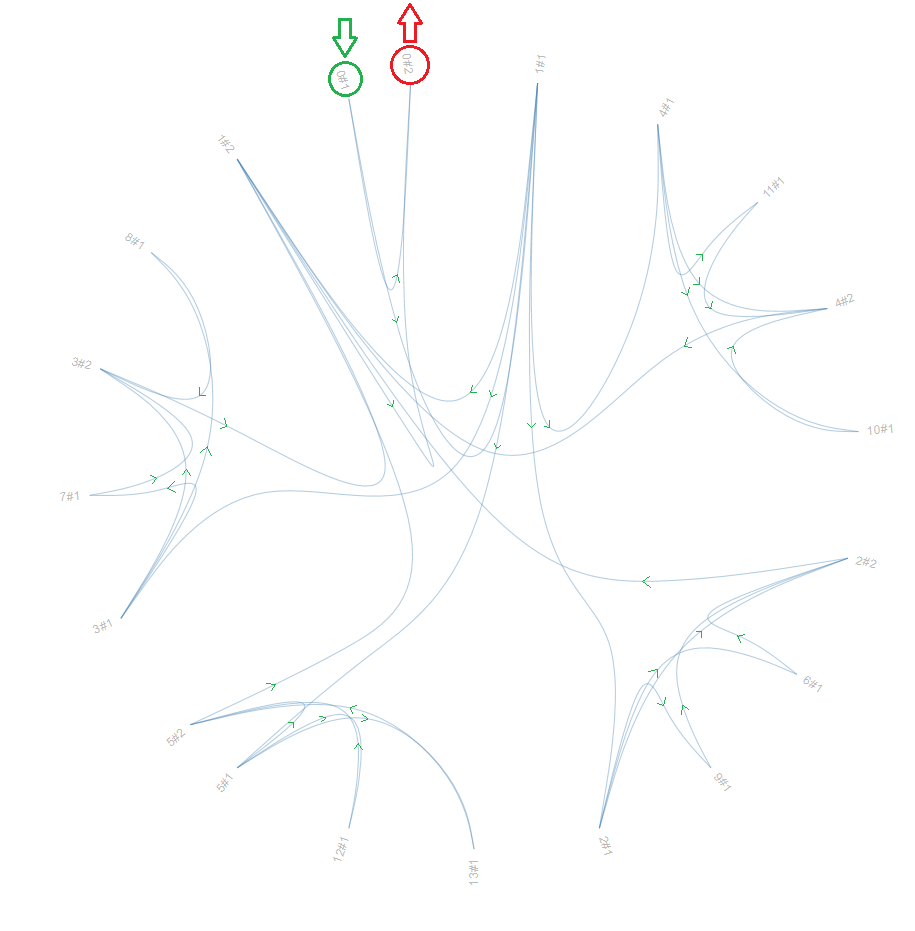
\includegraphics[width=1.4\textwidth]{bundle-fjt}}
  \caption{Fork-join algorithm dependency graph}
  \label{fig:fjt-bundle}
\end{figure}


\section{Transparent Instrumentiation with AspectJ}



\begin{itemize}
\item analysis
\item ralization
\item result
\end{itemize}

